\documentclass[a4paper,english,12pt]{article}
\usepackage{%
	amsfonts,%
	amsmath,%	
	amssymb,%
	amsthm,%
%	babel,%
	bbm,%
	%biblatex,%
	caption,%
	centernot,%
	color,%
	enumerate,%
	epsfig,%
	epstopdf,%
	etex,%
	geometry,%
	graphicx,%
	hyperref,%
	latexsym,%
	mathtools,%
	multicol,%
	pgf,%
	pgfplots,%
	pgfplotstable,%
	pgfpages,%
	proof,%
	psfrag,%
	subfigure,%	
	tikz,%
	ulem,%
	url%
}	

\usepackage[mathscr]{eucal}
\usepgflibrary{shapes}
\usetikzlibrary{%
  arrows,%
  backgrounds,%
  chains,%
  decorations.pathmorphing,% /pgf/decoration/random steps | erste Graphik
  decorations.text,%
  matrix,%
  positioning,% wg. " of "
  fit,%
  patterns,%
  petri,%
  plotmarks,%
  scopes,%
  shadows,%
  shapes.misc,% wg. rounded rectangle
  shapes.arrows,%
  shapes.callouts,%
  shapes%
}

\theoremstyle{plain}
\newtheorem{thm}{Theorem}[section]
\newtheorem{lem}[thm]{Lemma}
\newtheorem{prop}[thm]{Proposition}
\newtheorem{cor}[thm]{Corollary}

\theoremstyle{definition}
\newtheorem{defn}[thm]{Definition}
\newtheorem{conj}[thm]{Conjecture}
\newtheorem{exmp}[thm]{Example}
\newtheorem{assum}[thm]{Assumptions}
\newtheorem{axiom}[thm]{Axiom}

\theoremstyle{remark}
\newtheorem{rem}[thm]{Remark}
\newtheorem{note}[thm]{Note}

\newcommand{\norm}[1]{\left\lVert#1\right\rVert}
\newcommand{\indep}{\!\perp\!\!\!\perp}
\DeclarePairedDelimiter\abs{\lvert}{\rvert}%
%\DeclarePairedDelimiter\norm{\lVert}{\rVert}%
\newcommand{\tr}{\operatorname{tr}}
\newcommand{\R}{\mathbb{R}}
\newcommand{\Q}{\mathbb{Q}}
\newcommand{\N}{\mathbb{N}}
\newcommand{\E}{\mathbb{E}}
\newcommand{\Z}{\mathbb{Z}}
\newcommand{\B}{\mathscr{B}}
\newcommand{\C}{\mathcal{C}}
\newcommand{\T}{\mathscr{T}}
\newcommand{\F}{\mathcal{F}}
\newcommand{\G}{\mathcal{G}}
%\newcommand{\ba}{\begin{align*}}
%\newcommand{\ea}{\end{align*}}

% Debug
\newcommand{\todo}[1]{\begin{color}{blue}{{\bf~[TODO:~#1]}}\end{color}}


\makeatletter
\def\th@plain{%
  \thm@notefont{}% same as heading font
  \itshape % body font
}
\def\th@definition{%
  \thm@notefont{}% same as heading font
  \normalfont % body font
}
\makeatother
\date{}
 
\title{\textbf{Probabilistic Seismic Hazard Analysis}}
\author{Nazeeh K M and Ankit Tripathi}

\begin{document}
\maketitle

\section{Motivation}
Earthquakes are always associated with uncertainties in its time of occurrence, location of occurrence and its magnitude. This makes it inevitable to use probabilistic methods of analysis, so that such uncertainties can be considered and quantified, which helps in earthquake resistant design.
\section{System Model}
Probabilistic seismic hazard analysis (PSHA) provides a framework to account for the uncertainties in the estimation of seismic design parameters. The methodology uses the probabilistic concepts to identify, quantify and combine the uncertainties in size, location and rate of recurrence of earthquake. PSHA can be summarized in the following steps.
\begin{enumerate}
\item Identification and characterization of earthquake sources. considering the probability distribution of potential rupture locations within the source.
\item Characterization of temporal distribution of earthquake recurrence using recurrence relationship.
\item Determination of ground motion parameter using predictive relationship considering the inherent uncertainty in the relationship.
\item Combine the uncertainties in earthquake location, size and ground motion parameter prediction to obtain the probabilistic estimation of exceedance of the ground motion parameter during the time period under consideration.
\end{enumerate}
\section{Problem Statement}
Illustration of PSHA for the determination of ground motion parameters and rate of recurrence considering the uncertainties in location, size and time of occurrence, for a line source.
\subsection{Justification}
Deterministic analysis cannot account for the uncertainties associated with earthquake in its size, location and time of occurrence, which are inherent in the estimation and prediction of the seismic design parameters. When these uncertainties become significant, the error in the estimation also becomes significant. Under such circumstances PSHA can provide a probabilistic estimate of the design parameters, which will be more sensible.
\section{Spatial Uncertainty}
The geometry of the source depend on the tectonic processes involved. It can be a point source, one-dimensional line source, two-dimensional areal source or even three-dimensional volumetric sources. For characterizing the location of the source, the earthquakes are assumed to be uniformly distributed within a source. When sufficient data is available, non-uniform distributions as appropriate can be used as well. The uncertainty in source-to-site distance, $r$ is described by probability density function, $f_R (r) dr$.

\begin{figure}[h!]
\graphicspath{ {images/} }
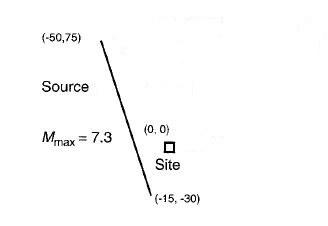
\includegraphics[width=\textwidth]{source}
\caption{Source and site location}
\label{figure:Source}
\centering
\end{figure}

In the present study a line source as shown in Figure $\ref{figure:Source}$ is considered, with a max earthquake magnitude of 7.3. From the geometry the shortest distance from the source to the site $r_min$ is calculated as $23.72 km$ and the length of the source $L_f$ is calculated as $90.14 km$. Therefore, the probability density function can be calculated as 

$$f_R (r) = \frac{r}{L_f \sqrt{r^2 - r_{min}^2}}$$

\begin{figure}[h!]
\graphicspath{ {images/} }
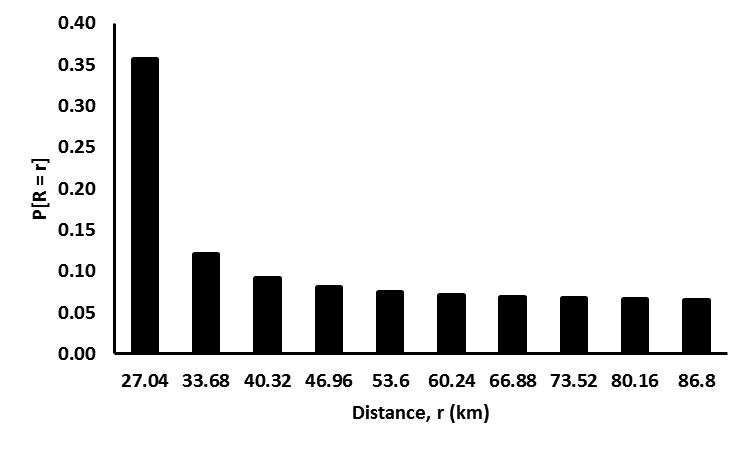
\includegraphics[width=\textwidth]{P_r}
\caption{Probability distribution of source-to-site distance}
\label{figure:distance}
\centering
\end{figure}

Figure $\ref{figure:distance}$ shows the probability distribution of source-to-site distance. 
\section{Size Uncertainty}
The distribution of earthquake sizes in a given period of time is described by recurrence law. Gutenberg-Richter Recurrence Law expresses the mean annual rate of occurrence as a function of the magnitude as per the following expression.

$$log \lambda_m = a - b m$$

where $\lambda_m$ is the mean annual rate of exceedance of magnitude, $m$ and $a$ and $b$ are constants that can be obtained by using the earthquake data over a time period at different magnitudes.

For the source considered in the present study, the recurrence law is given as

$$log \lambda_m = 4.4 - 1.0 m$$

All sources have a maximum earthquake magnitude that cannot be exceeded. In the present study it is $7.3 (m_u)$. And a minimum magnitude of $4 (m_l)$ is selected, below which the effect of the earthquake on the structures and utilities are negligible. Bounded Gutenberg-Richter Recurrence Law is used in the analysis, to determine the probability distribution of earthquake magnitude from the source considered.

$$P[m_l < m < m_u] = f_M (\frac{m_l + m_u}{2})(m_u - m_l)$$

Figure $\ref{figure:magnitude}$ shows the probability distribution of magnitude from the line source considered in the present study. 

\begin{figure}[h!]
\graphicspath{ {images/} }
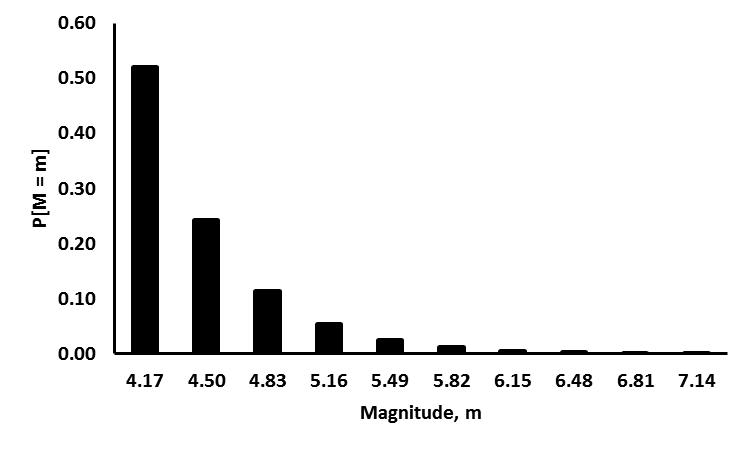
\includegraphics[width=\textwidth]{P_m}
\caption{Probability distribution of magnitude from the source}
\label{figure:magnitude}
\centering
\end{figure}
\section{Predictive Relationships}
Predictive relations are obtained by regression on strong motion parameter data. The scatter in the data is quantified by standard deviation or confidence intervals. Predictive relations give the ground motion parameters with respect to the magnitude and distance of the source. Predictive relationship given by Cornell et al. is used in the analysis.

$$ln PHA (gals) = 6.74 + 0.859 M - 1.80 ln (R + 25)$$

\section{Temporal Uncertainty}
Mean annual rate of exceedance of ground motion parameter - peak ground acceleration, is calculated by combining the uncertainties in source-to-site distance, magnitude and recurrence relationships. The temporal uncertainty in the occurrence is considered as Poisson model for illustration purpose in the present case. The seismic hazard estimated in terms of peak ground acceleration is hence combined with the Poisson model to estimate probabilities of exceedance in finite time intervals.

$$P[Y_t>y^*] = 1 - e^{\lambda_{y^*}T}$$

\begin{figure}[h!]
\graphicspath{ {images/} }
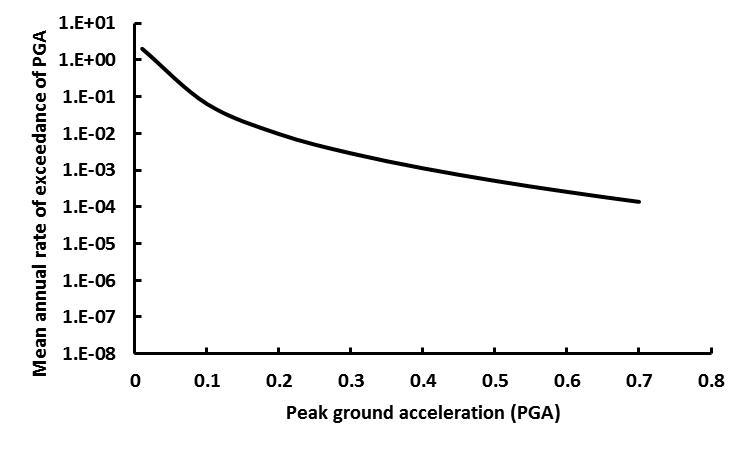
\includegraphics[width=\textwidth]{pga}
\caption{Seismic hazard curve for the line source}
\label{figure:pga}
\centering
\end{figure}

The value of ground motion parameter corresponding to a particular probability of exceedance $P$, in a given time period $T$, can be calculated by rearranging the previous equation.

$$\lambda _{y^*} = -\frac{ln(1 - P[Y_T > y^*])}{T}$$

From the seismic hazard curve given in Figure $\ref{figure:pga}$, using the mean annual rate of exceedance $\lambda _{y^*}$ calculated, peak ground motion parameter can be estimated. Figure $\ref{figure:time}$ shows the curve with mean annual rate of exceedance with a probability of $10\%$

\begin{figure}[h!]
\graphicspath{ {images/} }
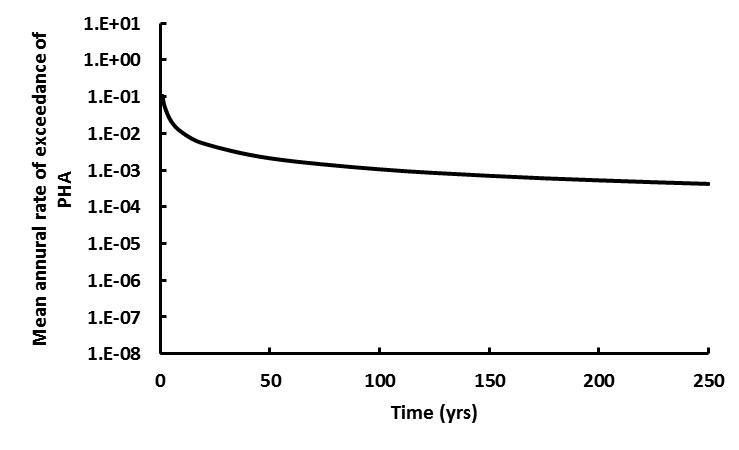
\includegraphics[width=\textwidth]{time}
\caption{Mean annual rate of exceedance with $10\%$ probability}
\label{figure:time}
\centering
\end{figure}
\subsection{Other Models}
Earthquakes are expected to happen due to release of the strain energy accumulated in the rocks due to tectonic movements. Under such circumstances the assumption of independent occurrence of earthquake may not be adequate. Further, the occurrence of a large earthquake should substantially reduce the chances of another independent, large earthquake occurring shortly thereafter from the same source. In such cases, there should be an attempt to use other models for probabilistic seismic analyses. 

There are different stochastic models available that account for prior seismicity.
\begin{itemize}
\item \textbf{Non-homogeneous Poisson models} allow the annual rate of exceedance to vary with time.
\item \textbf{Renewal models} use arrival time distributions other than exponential to allow the hazard rate to increase with time since the last event; Gamma and Weibull distributions are the most common.
\item \textbf{Time-predictable models} specify a distribution of the time to the next earthquake that depends on the magnitude of the most recent earthquake.
\item \textbf{Slip-predictable models} consider the distribution of earthquake magnitude depend on the time since the most recent earthquake.
\item \textbf{Markov models} incorporate a type of memory that describes the chances that a process moves from some past state to a particular future state. The time for which the process stays in a particular state before moving to another state is exponentially distributed.
\item \textbf{Semi-Markov models} are not restricted to exponential distribution. They can relate the probability of future earthquakes of various sizes to the size of the most recent event and the elapsed time since its occurrence.
\item \textbf{Trigger models} can account for clusters of events that occur after triggering events.
\end{itemize}
\subsection{Model Applicability}
Examination of past studies on the use of Poisson model in seismic hazard analysis shows that in most cases its application is appropriate and practical. The simplicity of Poisson model, its ease of use and lack of sufficient data to support more sophisticated models, also have contributed to the wide applicability of Poisson model.

However, when the seismic hazard is controlled by a single source with an elapsed time since the last event greater than the average inter-event time or for sources exhibiting strong characteristic earthquake behavior, it is not appropriate to use Poisson model. In these cases, it is more appropriate to use models that can capture the broader process of earthquake occurrence that includes memory of prior events in the assessment of future earthquake occurrence rates.

Each of the more sophisticated models uses a pattern of earthquake occurrence to reconcile their computed probabilities with the mechanics of the elastic rebound process of earthquake generations. As a result, each requires additional parameters whose values must be evaluated from the seismic records. The scarcity of data limits the accurate evaluation of these additional parameters. As additional data becomes available, the applicability and use of these models will be higher.
\section{Summary}
The present study illustrates Probabilistic Seismic Hazard Analysis of a site due to a line source. The uncertainties regarding location, magnitude, predictive relations and the occurrences of earthquakes are considered under the framework of PSHA. The seismic hazard curve and the mean annual rate of exceedance of peak ground motions for a given probability of exceedance under different time periods provided can be used in seismic resistant design.

In the illustration of PSHA, temporal uncertainty is considered by using a Poisson model for earthquake occurrence. An overview of other models available and their applicability is also provided as a discussion.
\section{References}
\begin{enumerate}
\item Kramer, S. L., (1996) $"Geotechnical Earthquake Engineering"$ University of Washington. Prentice-Hall International Series in Civil Engineering and Engineering Mechanics.
\end{enumerate}
\end{document}